\documentclass[11pt,a4paper]{article}

\usepackage[utf8x]{inputenc}   % omogoča uporabo slovenskih črk kodiranih v formatu UTF-8
\usepackage[slovene]{babel}    % naloži, med drugim, slovenske delilne vzorce

\usepackage{graphicx} % omogoča vključevanje slik


\title{Poročilo seminarske naloge - Seam Carving}
\author{Žiga Strgar\\
zs1429@student.uni-lj.si\\
\ \\
Fakulteta za računalništvo in informatiko Univerze v Ljubljani
\date{\today}
}


\begin{document}
\maketitle

\section{Opis problema}

Pri krčenju slik se zoprestavimo s problemom, kako zmanjšati sliko brez da iz
nje izgubimo kakšen pomemben podatek. Če uporabimo tehniko "scale" se objekti
sploščijo, če izvajajmo operacijo samo na eni osi. Obrezovanje je tudi nezaželjeno
kajti izgubimo prvotno sliko, sploh pa če so pomembni elementi slike na samem robu.

Pri tem nam lahko pomaga \textbf{izrezovanje šivov} (\emph{ang. seam carving}).
Ne le da rešuje problem krčenja slik, nam lahko tudi pomaga pri večanju slike z
vstavljanjem šivov.

\section{Arhitektura in pristop}

\subsection{OpenCL}

Je ogrodje, ki omogoča računski, delovni ali podatkovni paralelizem na različnih
enotah (CPE, GPE, DSP, FPGA). Specificiran je v jezikih (C99 in C++11). Tako da
podpira nizkonivjsko programski vmesnik (API), ki nadzoruje in izvaja programe/ščepce
na omenjenih enotah. Je odprtokoden in v njegov razvoj prispevajo vsa večja
računalniška podjetja na svetu.

\subsection{Pristop}

\subsubsection{Serijsko}

Najprej pripravim vse potrebne spremenljivke, določim potrebne vrednosti in nato
preberem sliko s katero želim delati. Prvi korak je izračun oziroma izdelava
sobel slike, s pomočjo katere nato izračunam kumulative. Te računam od spodaj
navzgor. Sledi iskanje šiva, tega najdem tako da poiščem minimum v prvi vrstici,
kar pomeni da je to začetek šiva in ga nastavim na -1, nato pa se v zanki
 sprehodim čez višino slike in gledam 3 pixle (levi, sredinski, desni),
 pogledam kater je najmanjši od teh treh in tja zapišem -1. Nato pa prepisujem
 sliko tako, da preskakujem vrednosti -1, kar pomeni da te pixle odstranim
 iz slike. To ponovim toliko krat kolikor šivov želim odstraniti. Rezultat po
 vseh iteracijah shranim nazaj v sliko.

\subsubsection{Paralelno}

Prvo pripravim vse spremenljivke in preberem sliko s katero delam. Sledi branje
kernel.cl datoteke, kjer se nahaja OpenCL koda s tremi "kerneli". En za izračun
oziroma izdelavo sobel slike. Drugi za izračun kumulativ iz sobel slike in iskanje
šiva, ki ga shrani v vektor velikosti višine slike. Zadnji pa za odstranitev
šiva iz slike. Sam postopek pa je enak kot v serijskem delu, le da se tu večina
stvari izvaja na GPU.

\section{Strojna oprema}

Program sem poganjal na računalniku Macbook Pro s procesorjem Intel i5 (\emph{2,7 GHz}).
Nima pa ločene grafične kartice, zato sem drugi del naloge opravljal na Intel Iris 6100
grafičnem čipu, ki si deli 1,5 GB DD3 pomnilnika s sistemom. Hitrost pomnilnika
dosega \emph{1867 MHz}.

\pagebreak

\section{Časi izvajanja in primerjave}

Vsi časi so povprečje 10ih meritev na CPE in GPE v sekundah. Merjeni s pomočjo
knjižnice \emph{omp.h}. Vsi programi prevedeni z zastavico \emph{-O3}.

\subsection{Broadway tower}

Slika velikosti $1428 \times 968$ pixlov.

\begin{figure}[htb]
\begin{center}
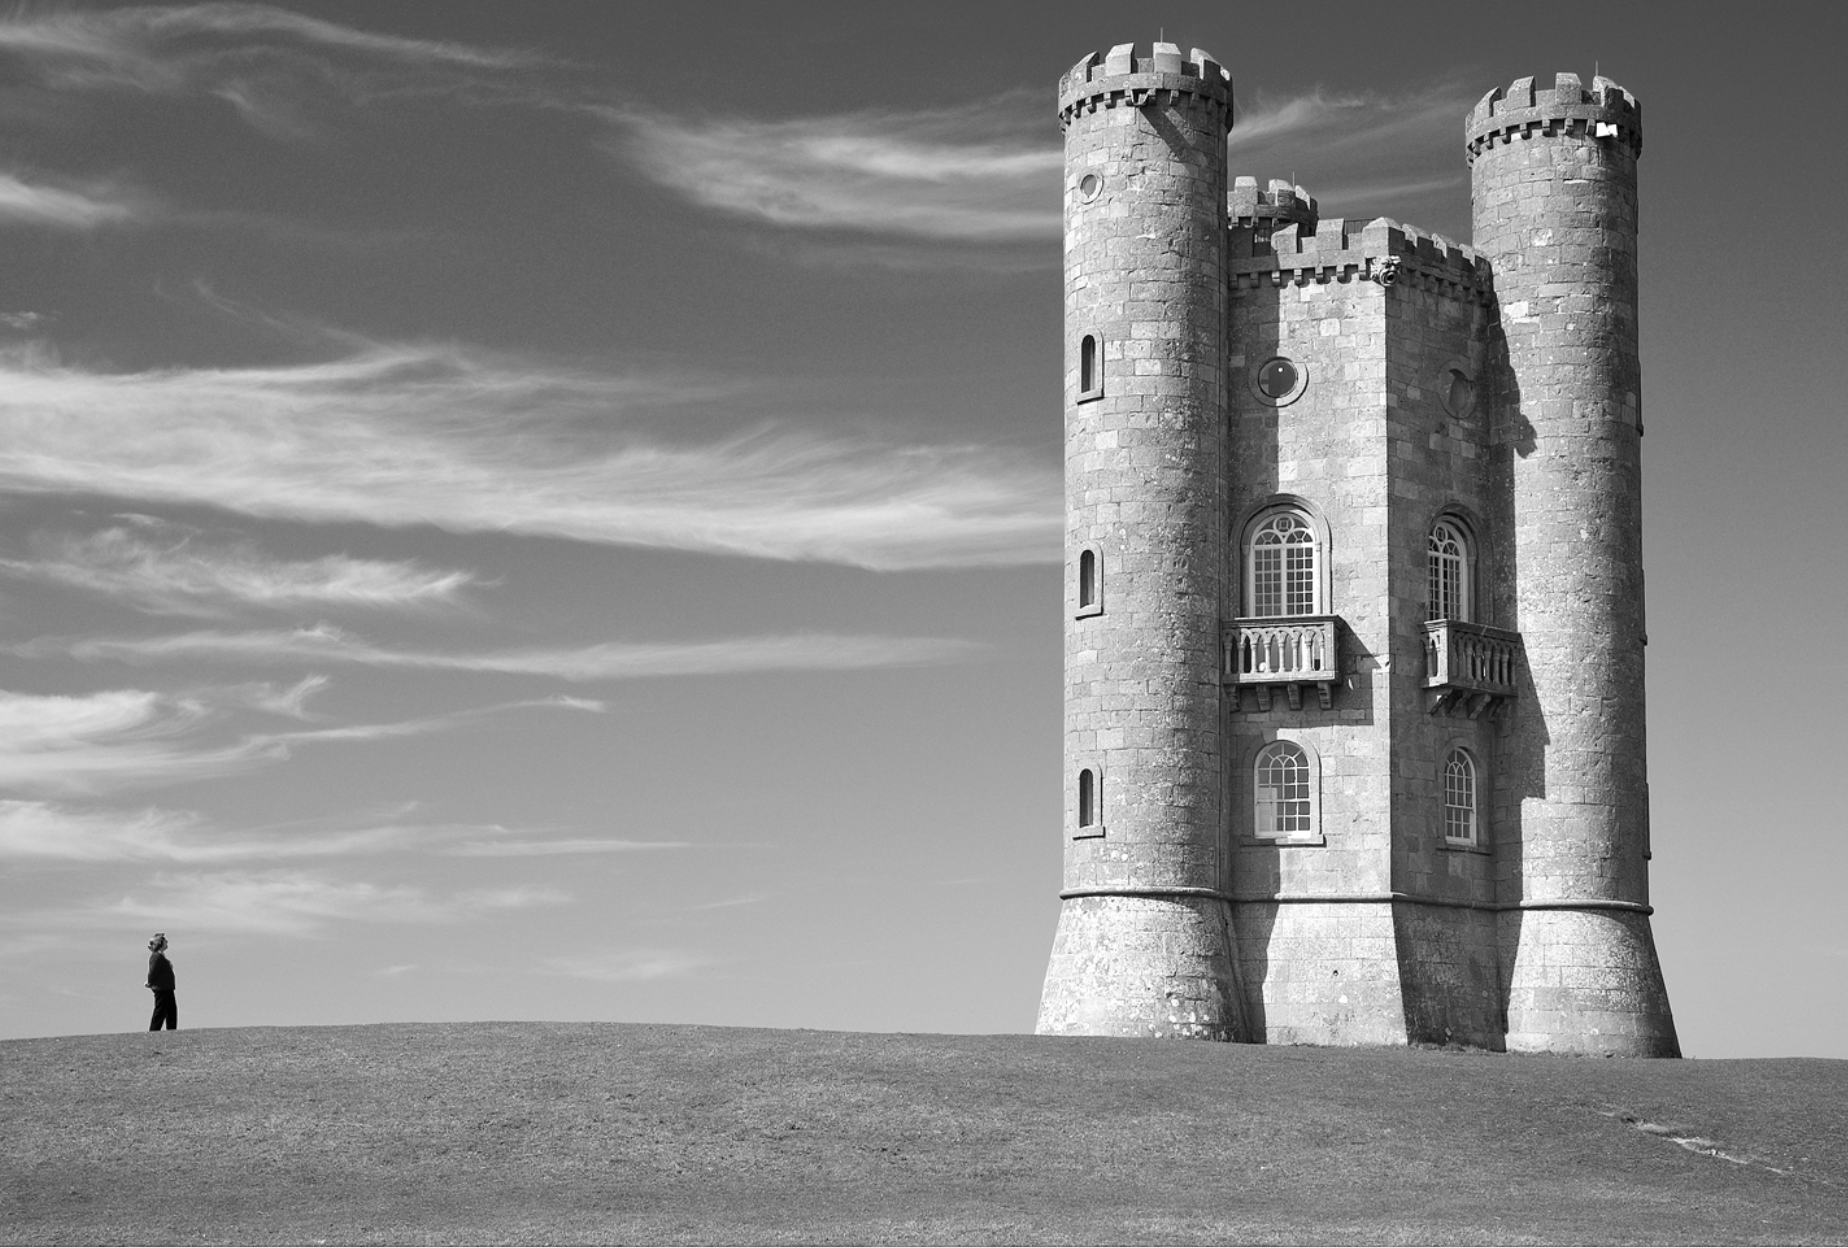
\includegraphics[width=0.7\columnwidth]{tower_original.png}
\end{center}
\caption{Broadway tower originalna slika}
\label{fig:tower_original}
\end{figure}

\begin{center}
  \begin{tabular}{ c | c | c | c }
    Število odstranjenih šivov & Čas CPE & Čas GPE & Faktor pohitritve \\
    \hline
    10 & 0.316394 & 0.123355 & 2.564 \\
    50 & 1.536728 & 0.576643 & 2.664 \\
    100 & 2.995582 & 1.126542 & 2.659 \\
    200 & 5.723353 & 2.149746 & 2.662 \\
    300 & 8.223347 & 3.0986945 & 2.653 \\
    \hline
  \end{tabular}
  \caption{Izmerjeni časi in faktor pohitrtive za sliko Broadway tower}
  \label{tab:performance_tower}
\end{center}

\begin{figure}[htbp]
\begin{center}
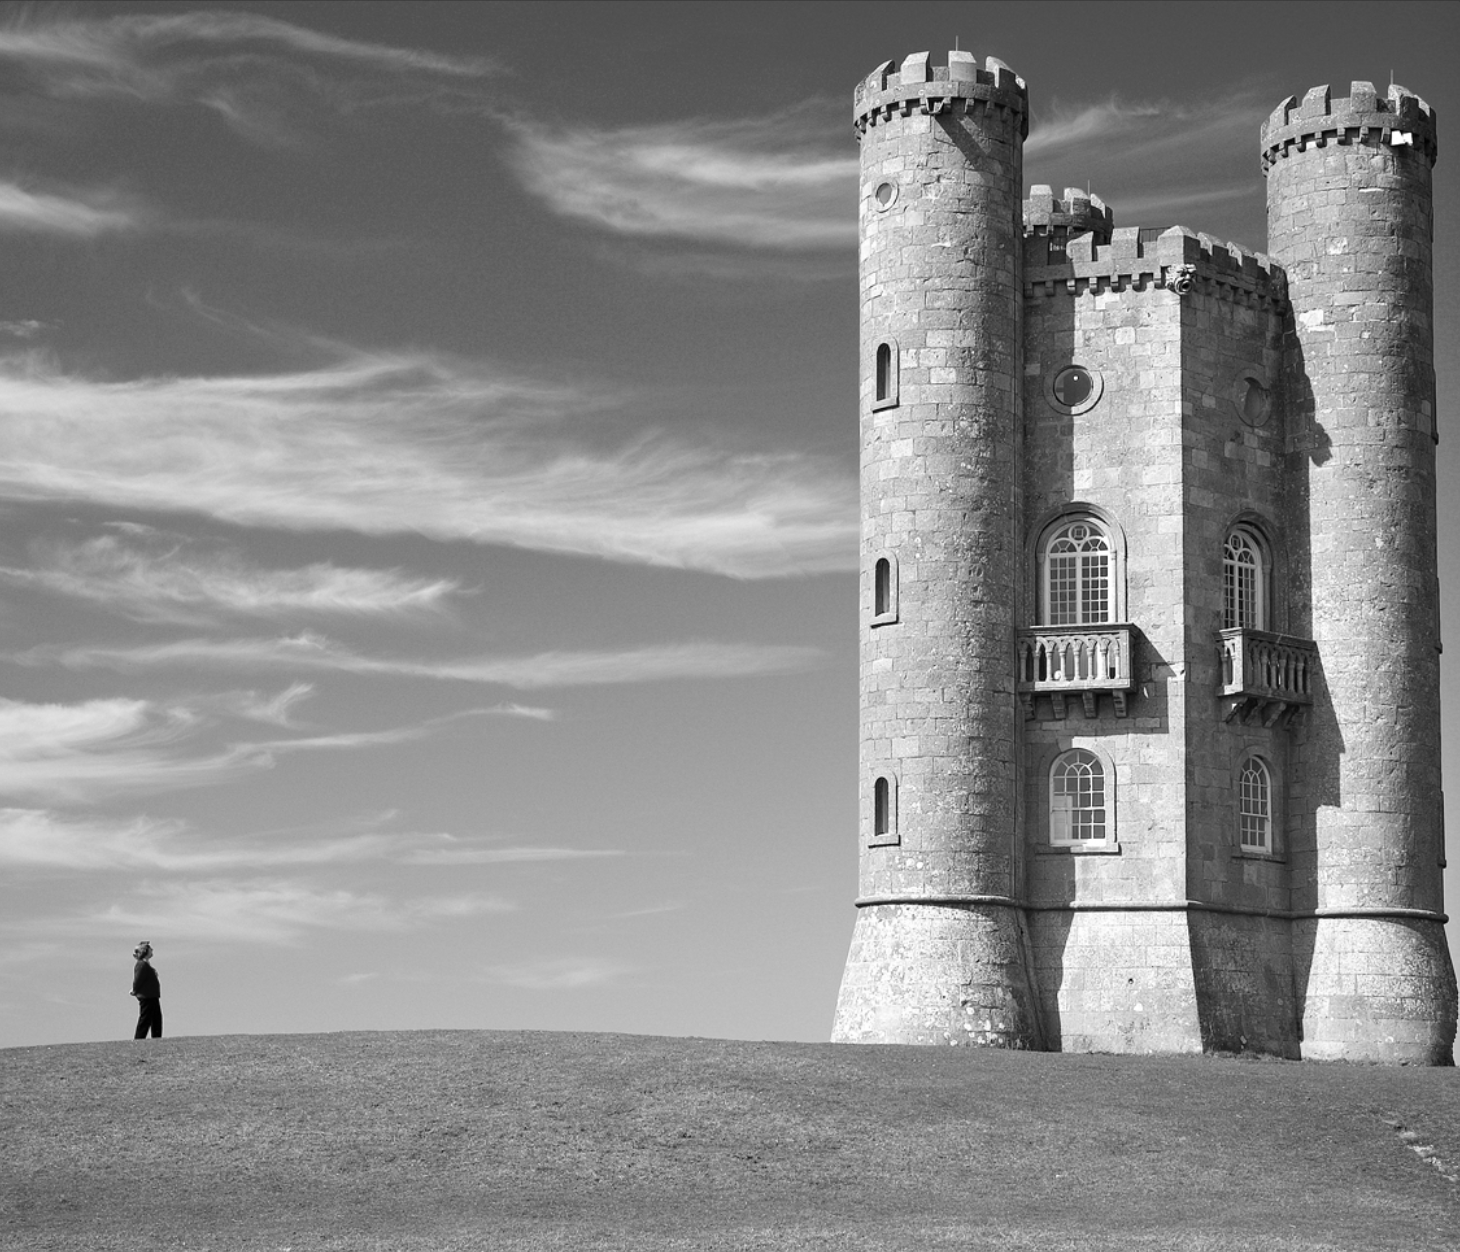
\includegraphics[width=0.7\columnwidth]{tower_100.png}
\end{center}
\caption{Broadway tower z odstranjenimi 100 šivi na CPE}
\label{fig:tower_seam}
\end{figure}

\pagebreak

\subsection{Eidsvatnet jezero, Norveška}

Slika velikosti $5177 \times 3456$ pixlov.

\begin{center}
  \begin{tabular}{ c | c | c | c }
    Število odstranjenih šivov & Čas CPE & Čas GPE & Faktor pohitritve \\
    \hline
    10 & 4.0657288 & 1.2505322 & 3.251 \\
    50 & 20.233545 & 6.6923732 & 3.023 \\
    100 & 38.943393 & 13.04972 & 2.984 \\
    200 & 80.580615 & 25.7609367 & 3.128 \\
    300 & 117.785656 & 38.3618806 & 3.070 \\
    \hline
  \end{tabular}
  \caption{Izmerjeni časi in faktor pohitrtive za sliko Eidsvatnet}
  \label{tab:performance_eidsvatnet}
\end{center}

\begin{figure}[htb]
\begin{center}
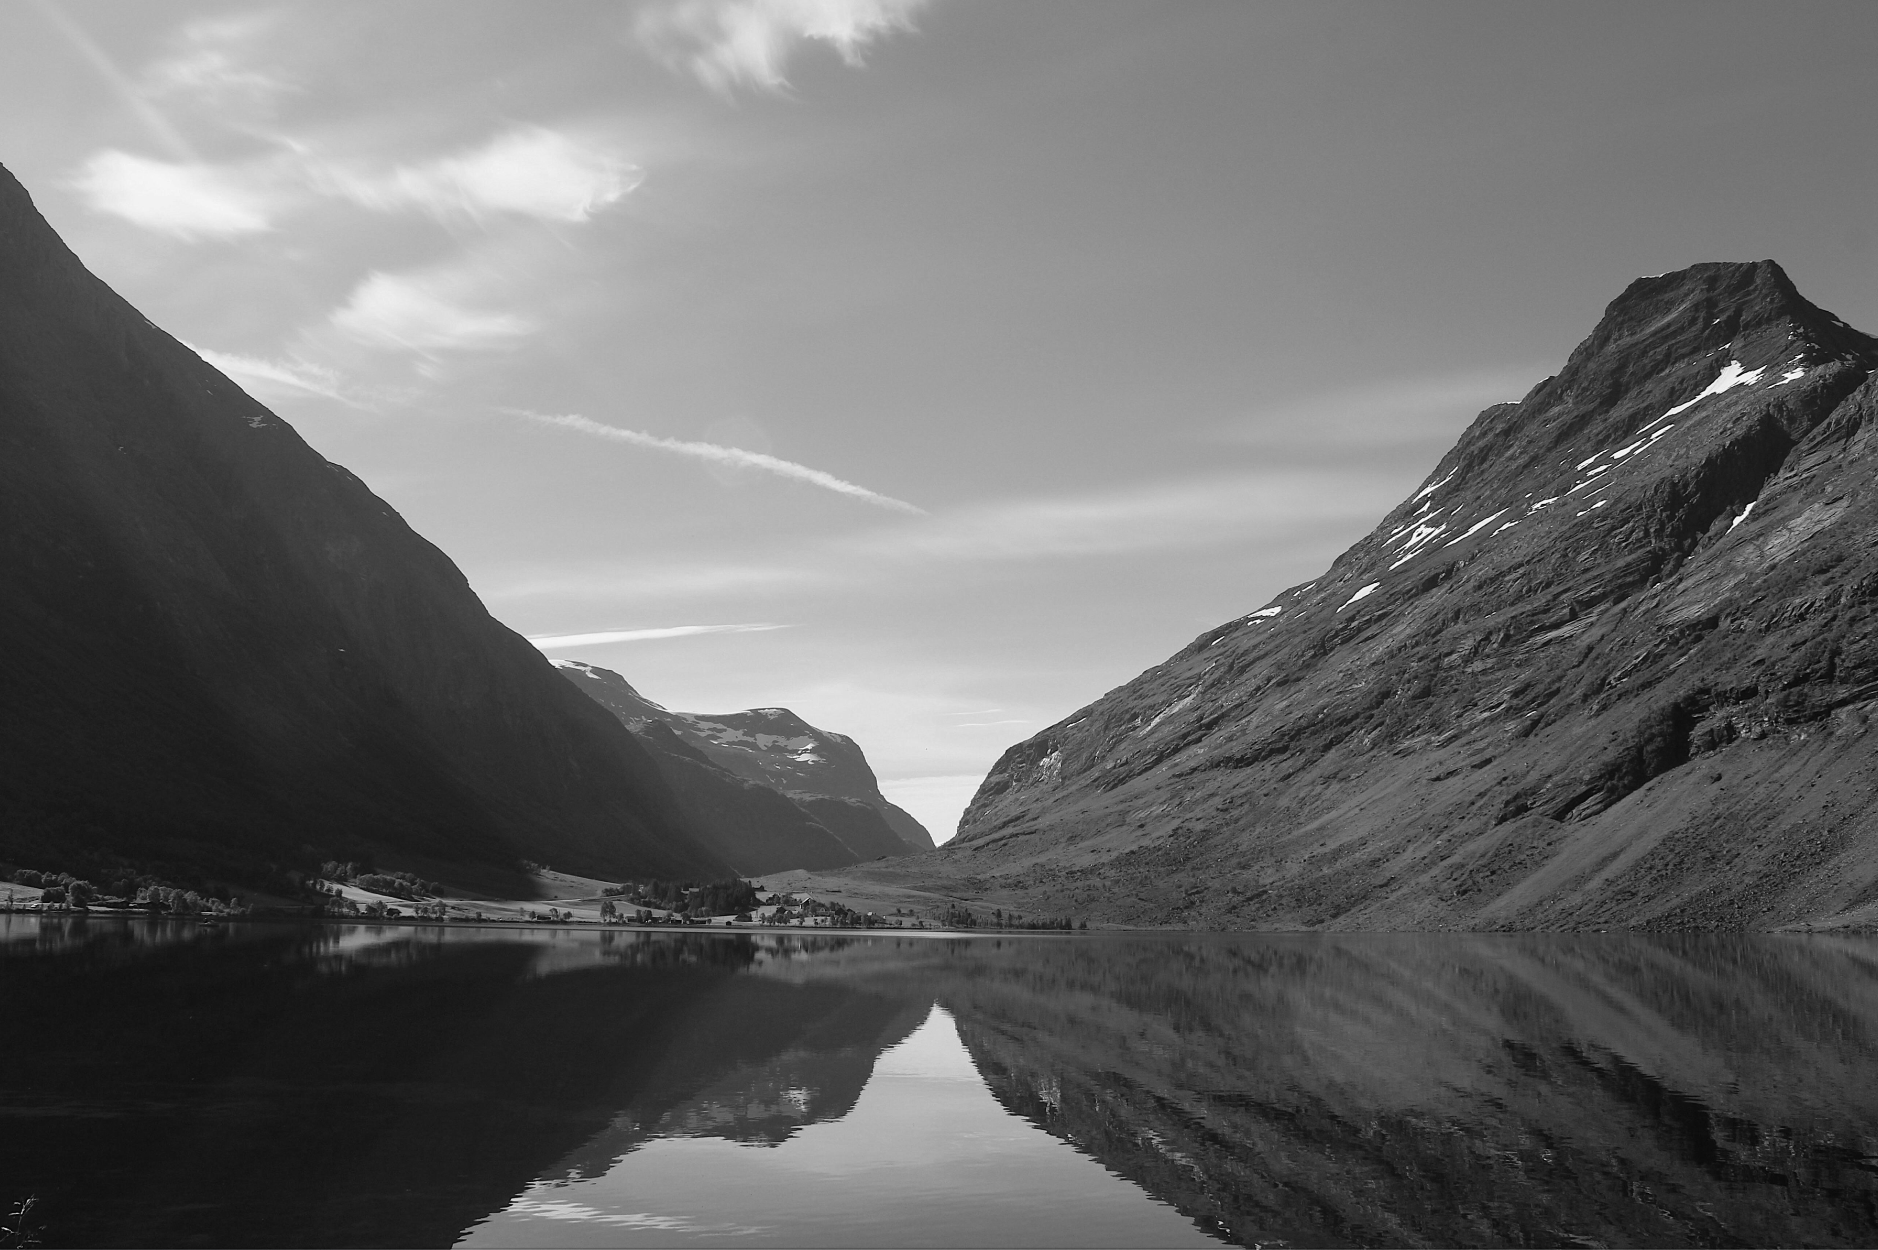
\includegraphics[width=0.6\columnwidth]{eidsvatnet_original.png}
\end{center}
\caption{Eidsvatnet originalna slika.}
\label{fig:eidsvatnet_original}
\end{figure}

\begin{figure}[htb]
\begin{center}
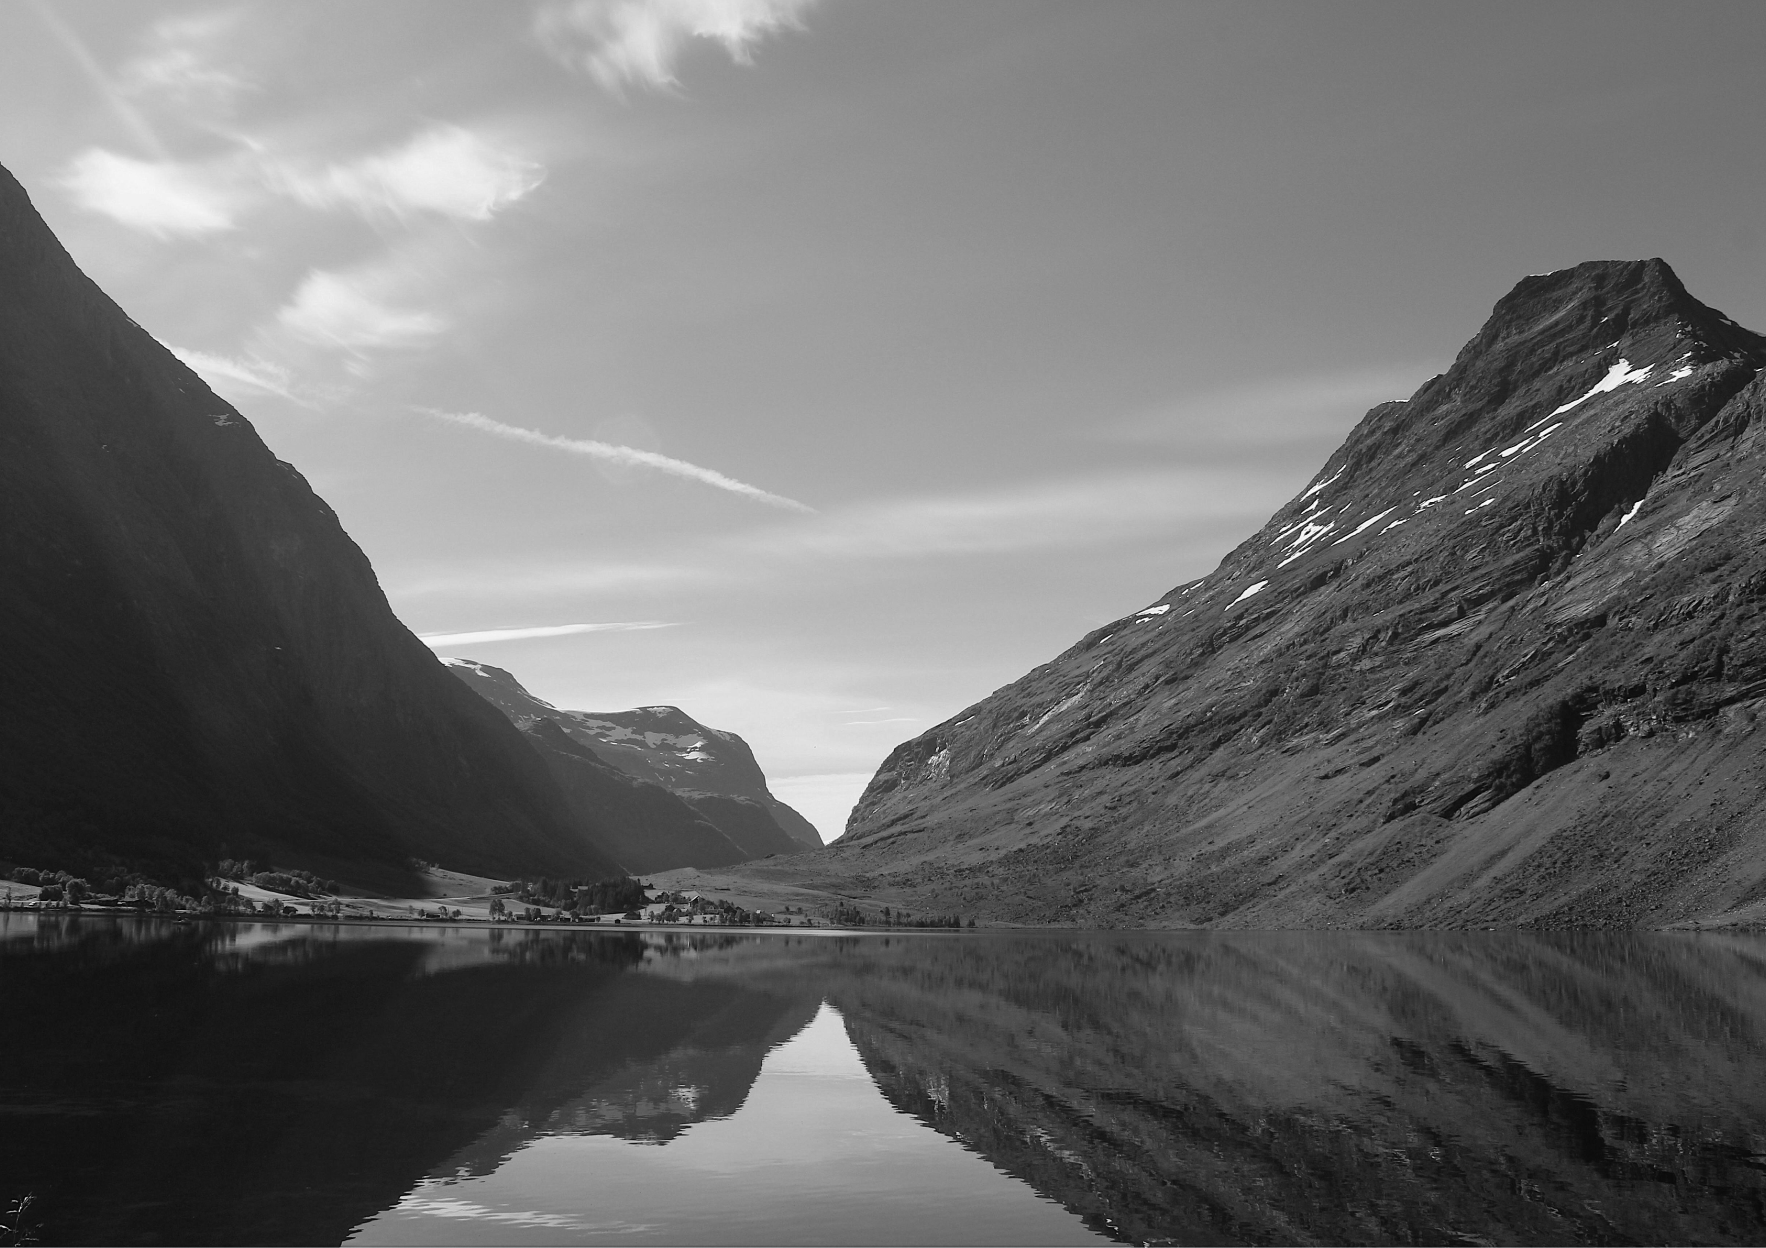
\includegraphics[width=0.6\columnwidth]{eidsvatnet_seam.png}
\end{center}
\caption{Eidsvatnet s 300 odstranjenimi šivi na GPE}
\label{fig:eidsvatnet_seam}
\end{figure}

\pagebreak

\subsection{Uporaba \_\_local}

Pri uporabi lokalnega deljenega pomnilnika pri računanju sobel-a se povprečni
čas zmanjša zgolj za 0.897667s. To sem testiral na sliki Eidsvatnet s 300
odstranjenimi šivi.

\section{Posebnosti implementacije}

Večjih posebnosti v moji implenentaciji ni. Omenil pa bi da pri paralelnem delu
kode menjam kje je začetna slika in kje lokacija končne slike. To delam zgolj
zato, da ne kopiram rezultat odstanjevanja šiva nazaj na lokacijo, kjer je
original slika. Temveč uporabim kar to končno sliko in v tej iteraciji nato
uporabim za lokacijo končne slike kar lokacijo prvotnega originala, in tako menjam
vsako iteracijo.

\section{Možne nadgradnje}

Uporaba lokalnega pomnilnika tudi pri računanju kumulativ.

\section{Ugotovitve}

Pohitritev na GPE je v primerjavi s CPE kar nekako konstanta ne glede na število
odstranjenih šivov. Najmanjša razlika je seveda pod 10 rezanih šivov, vse ostalo
pa kar primerljivo. Seveda pa dosežemo veliko višjo pohitritev z čim večjo
fotografijo, ki jo želimo obdelati. Dosežemo pa lahko tudi več kot 3x pohitritev
 v primerjavi s CPE.

\end{document}
